\section{Velocity controller test}
A velocity tests has been done to prove that the velocity changes dependant to the distance from a person to the robot. When the distance is 1.2m the velocity should be at its highest and when the distance is close to 3m, the velocity should decrease to minimum and stop. This tests also shows whether or not the velocity is the value it has been programmed to be for the specific distances.\\

\textbf{Equipment}: The equipment used for executing the test is chalk to mark two lines, the robot used to move from one place to another and a timer.\\

\begin{figure}[H]
    \centering
    \begin{minipage}[b]{0.57\linewidth}
        \textbf{Setup}: The test is executed in a hallway where a goal line has been marked 4 meters from the start line, see figure \ref{fig:test_velocity_setup}.
        The robot is placed a bit before the start line and has to move across the goal line. The two lines has been marked on the floor with chalk and has to be clear to see for us to be able to determine when the robot has passed the line.\\
        
        \textbf{Execution}: Beginning the test, we tell the program what the distance from the robot to the human is. There is no actual human needed for following the robot in this test, since the program is told that there is one and with this static distance, a specific time is predicted as a result. When the distance is set to 1.2m, the robot is expected to have a velocity of 0.704m/sec. When the distance is set to 1.3m, the robot is expected to have a velocity of 0.666m/sec. These velocities has been pre-programmed to a specific distance with an algorithm. %This test is to confirm that the velocity will drop when the distance from human to robot increases.
        
    \end{minipage}
    \hspace{0.2cm}
    \begin{minipage}[b]{0.4\linewidth}
        \centering
        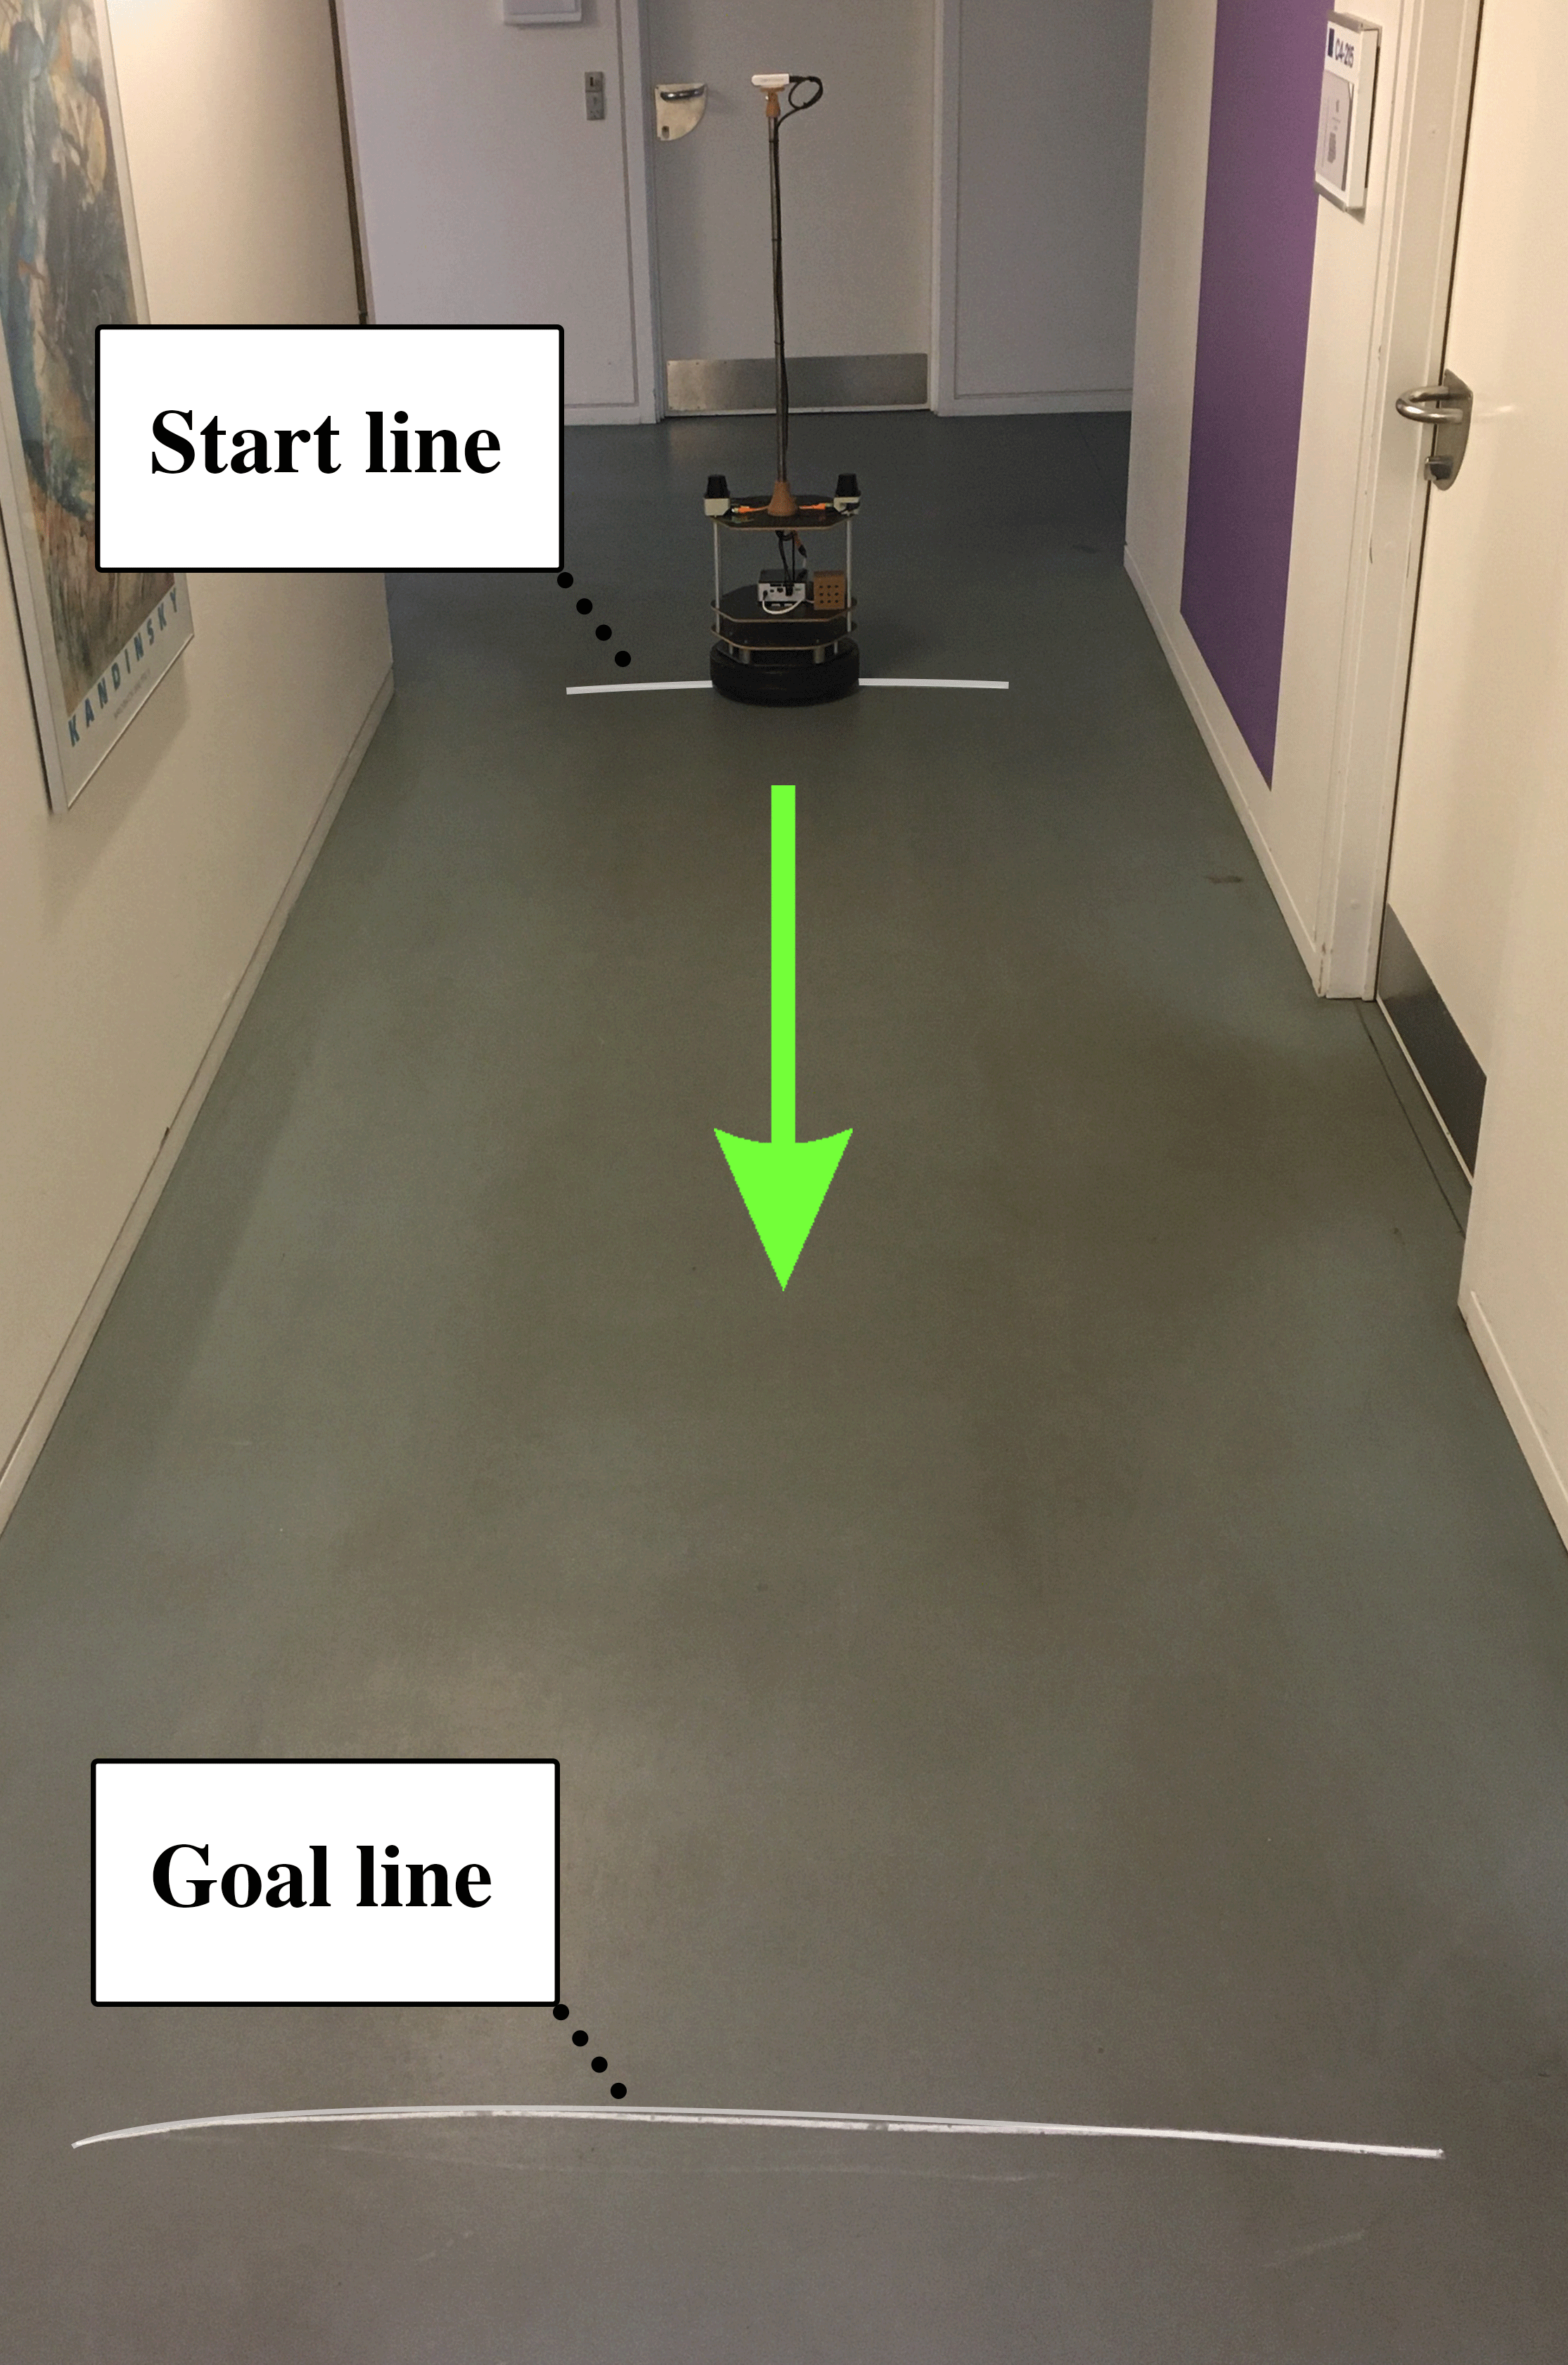
\includegraphics[width=\textwidth]{figures/velocityTest.png}
        \caption{Image showing the setup of the robot standing on the starting line ready to go to the goal line. There is 4 meters between the two marked lines.}
        \label{fig:test_velocity_setup}
    \end{minipage}
\end{figure}
The robot, which is placed a bit before the start line, is being told to move to a point across the goal line, via the software called RViz. When the robot's center crosses the start line, we manually start the timer and manually stop it as the center of the robot crosses the goal line. This has been done two times with ten different static distances to the robot. These different velocities can be seen on figure \ref{fig:test_velocity_setup}.\\

\textbf{Test parameters}: The time it takes for the robot to reach the goal line from the starting line, can be used for calculating if the velocity is behaving like wanted to in relation to the distance.\\

\textbf{Results and analysis}: Both the first and the second test result for all distances can be found in appendix \ref{} and the calculated average of the two can be seen on figure \ref{fig:TableVelocity}. \textit{Calculated distance} from the figure is calculated by \textit{Velocity}*\textit{Average time}, which is the distance it should have moved, if the given velocity was correct. Why the distance is more than 4m as it should not have been, is explained later under \textit{Sources of error}. \textit{Actual velocity} has been calculated by dividing the testing distance of 4m and the average time, such as $4/9.30=0.430$. This shows what velocity the robot actually had when moving.

\begin{figure}[H]
    \centering
    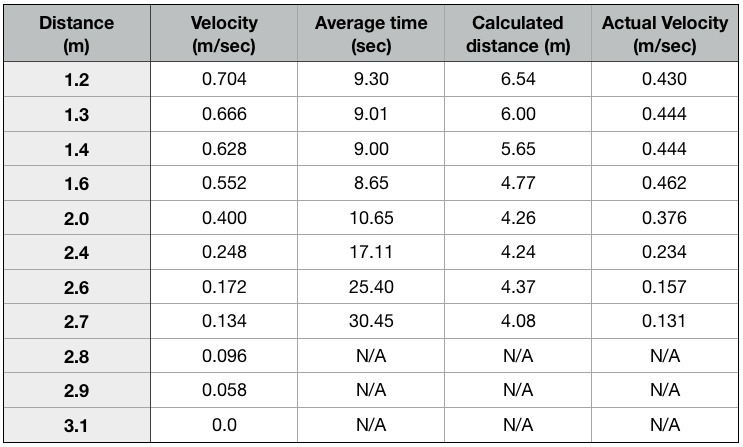
\includegraphics[width=\textwidth]{figures/velocity1.png}
    \caption{Results of the velocity test.}
    \label{fig:TableVelocity}
\end{figure}

When the distance was at its shortest of 1.2m, the velocity was at its highest, which should have been 0.704m/sec. Here the robot started to jiggle and could not keep up because of the hardware. When the distance was higher than 2.7m the robot started turning around itself very slowly and did not go forward, also because of the hardware. Since it could not move from the start line to the goal line, there are no result numbers for \textit{Average time}, \textit{Calculated distance} or \textit{Actual velocity} when the distance becomes too high.\\

\textbf{Sources of error}:
\begin{itemize}
    \item The distance between the two chalk lines are 4m $\pm 1cm$ and the imprecision may have affected the result.
    \item The timer was operated by a person and the response time of pushing the start/stop button may not have the highest precision and was also the reason for taking two tests of each distance.
    \item The payload of the robot was not considered when sending velocity commands and could have affected the time and is also one reason for the imprecision in \textit{Expected distance}.
    \item The floor surface could cause slippage of the wheels and as such it would take longer time to reach the 4m distance than expected.
    \item The reason for the robot to spin around itself could also be the payload of the robot was too high to move the robot with such a low given velocity.
\end{itemize}